% \subsection{Characterization of Performance}

Before embarking in a computational campaign that will consume 150M core
hours on the NCSA Blue Waters machine, we study the scalability of the ESMACS
protocol to determine optimal workflow sizing and resource utilization. The
goal is twofold: (1) understanding the invariance of HTBAC execution time
over the number of workflow pipelines executed; and (2) studying how
EnTK---the RCT tool responsible for coordinating the distributed execution of
the protocol---scales its performance in relation to the size of HTBAC
workflow.

% ---------------------------------------------------------------------------
\subsubsection{Experiment Design}

We designed two experiments to measure HTBAC and EnTK weak scalability when
executing an increasing number of concurrent pipelines. According to the use
case described in Section~\ref{sec:ht-bac}, each pipeline consists of seven
stages, each stage with a single task. EnTK manages the queuing of the tasks
in accordance with the order and concurrency mandated by stages and
pipelines: For each pipeline, each stage is executed sequentially while
pipelines are executed concurrently.

\mtnote{PLease note: I converted the following paragraph eliminating
references to RP\@. This is consistent with out decision of not showing RP
overheads. The paragraph can be reused if we change our mind. ``
We validate the performance of EnTK % the runtime system, RADICAL-Pilot, 
using weak scalability to to show % demonstrate 
that EnTK % RP 
can schedule tasks concurrently, provided that sufficient resources are
available.''}\jhanote{+1}


Experiment 1 measures the baseline behavior of EnTK with the HTBAC workflow
and a null payload (\textmd{/bin/sleep 0}). The goal is to isolate the
overheads of EnTK from the specifics of: (1) the executables of the HTBAC
workflow; (2) the runtime used to execute the workflow on the HPC resources;
and (3) the overheads of the resources. The null workload does not require
data staging, I/O on both memory and disk, or communication over network.

Experiment 2 replicates the design of Experiment 1 but it executes the HTBAC
workflow with the use case payload. The comparison between the two
experiments enables performance analysis of EnTK to understand whether and
how the size of the executed workflow affects its overheads. Further,
Experiment 2 shows also whether HTBAC is sensitive to the number of
concurrent pipelines executed.

% In order to show % demonstrate 
% that % RP 
% EnTK is invariant to the type of workload, we run two types of experiments:
% We ran the HTBAC workflow with null workload in which each task did no work
% (/bin/sleep 0), the actual simulation workload. 

Both experiments measure the weak scalability of HTBAC and EnTK\@. This means
that the ratio between the number of pipelines and cores is kept constant by
design. While an investigation of strong scalability would contribute to a
better understanding of the behavior of both HTBAC and EnTK, it is of limited
interest for the current use case. The driving goal of HTBAC is to increase
throughput by means of concurrency, not of number of sequential execution per
core. This is one of the reasons because our project targets large HPC
machines instead of so-called HTC infrastructures.

% We illustrate the high throughput capabilities of the HTBAC workflow using
% ESMACS protocol by examining scalability in the number of pipelines and
% characterizing the performance of the workload. We show that the
% scalability we measure of the workflow is unrelated to the scalability of
% EnTK\@.

% ---------------------------------------------------------------------------
\subsubsection{Experiment Setup}

We perform both Experiment 1 and 2 % scalability experiments 
on the Blue Waters HPC cluster---a 13.3 petaFLOPS Cray at NCSA and University
of Illinois, with 32 Interlago cores/50 GB RAM per node, Cray Gemini, Lustre
shared file system. Currently, we exclusively use CPUs on Blue Waters as GPUs
are not required by our use case. RCTs support the use of both type of
architectures and we previously benchmarked the use of GPUs for later
evaluation.

% We characterize the weak scalability of the ESMACS protocol using Ensemble
% Toolkit running exclusively on Blue Waters CPUs.

We perform our experiments from a virtual machine hosted in Europe. This
helps to simulate the conditions in which the experimental campaign will be
performed by the research group at UCL\@. This is relevant because, as most
HPC resources, Blue Waters does not allow for executing applications on the
login node of the cluster. To this end, RCTs support \textmd{gsissh} for X509
authentication and authorization.

Table~\ref{tab:exp}\mtnote{to be done if we agree it would be useful} shows
the setup for Experiment 1 and 2. Currently, the ESMACS protocol is executed
with up to 25 concurrent pipelines. This number is suboptimal as pipelines
are independent and therefore their concurrent execution does not entail
communication overhead. Further, the system simulated can benefit from
concurrency because potential HTBAC users may require their use-case protocols extend 
the number of replicas beyond the current scale of ESMACS\@. Consistently, our
experiments push the boundaries of current scale by executing 8, 16, 32, 64
and 128 concurrent pipelines.

% requires The amount of replicas required by has an upper-bound of 25
% replicas yet we extend the number replicas to 128 in order to show higher
% scalability with a greater degree of confidence for the potential HTBAC
% user.

EnTK uses RADICAL-Pilot to acquire resources via a single pilot. 
% In the pilot description of EnTK, 
The size of the pilot is contingent upon characterization of performance, in
this case, weak % or strong scaling
scalability. % In the event of weak scaling we 
Accordingly, we % provide 
use the same number of cores in a pilot % the pilot size description 
as % the number of cores 
those required by the workload. 
% The number of cores is varied 
We use between 64 and 1024 cores in both Experiment 1 and 2, and we always
keep the number of simulations % is kept 
equal to the number of cores. % at all times. 
We 
% range the number of concurrent replicas % ranged
% from 8 to 128, % running concurrently using 
use either 1 or 8 cores per task % replica, 
depending on the task requirements.



\mtnote{The following needs discussion: ``The size of the workload is varied
in proportion to the amount of resources such that all tasks are concurrently
executed at all times.'' I believe this is not necessary true: we do not
execute all the tasks concurrently all the time but we always get enough
cores to run at least one task from each concurrent pipeline. Alternatively,
at every point in time, there are enough cores so that pipelines do not
compete for the same core.}\jhanote{I agree we do not run all the tasks
concurrently.}

\jdnote{in reference to above: This is not the case, we've determined that pipelines are indeed competing for resources because we have a round robin scheduler not the first-in-first-out scheduler. Therefore I'm amending this section: As we increase the number of pipelines, we increase the amount of resources by the same proportion for a given workload.}

\mtnote{I would represent the following with a table. Please feel free to
change it back if you disagree. ``For example, in the ESMACS protocol, the
simulation task specifies 8 cores per pipeline, therefore the pilot size is
defined as 8 \(\times \) number of pipelines. We vary the number of pipelines
to characterize weak scaling performance where the tasks are scheduled
concurrently.''}

\begin{table*}[t]
\centering
\caption{Experiment Setup}
\label{my-label}
\begin{tabular}{llllll}
\hline
\multicolumn{1}{l|}{Experiment ID \& Description} & \multicolumn{1}{l|}{Trials} & \multicolumn{1}{l|}{Pipelines} & \multicolumn{1}{l}{Stages} & \multicolumn{1}{l|}{Tasks} & \multicolumn{1}{l}{Total Number of Cores} \\ \hline
1 (Null)                                           & 2                           & 8, 16, 32, 64, 128             & 7                           & 7                          & 64, 128, 256, 512, 1024                    \\ \hline
2 (Use-Case)                                       & 2                           & 8, 16, 32, 64, 128             & 7                           & 7                          & 64, 128, 256, 512, 1024                    \\ \hline
\end{tabular}
\end{table*}

\mtnote{The following should probably moved to the next subsection, when
discussing the results of the experiments: ``For each of these
configurations, the simulation execution time is observed to be constant.''}
\jhanote{yes}

All the experiments use Ensemble Toolkit version 0.4.7 and RADICAL-Pilot
version 0.42. In the MD workload of the HTBAC workflow, the simulation tasks
are executed using NAMD-MPI\@. The equilibration % stages 
tasks of stage 4 and 6 are assigned 5000 timesteps while the task of stage 5
requires 55000 timesteps. We ran both the null and MD workload for two trials at each pipeline configurations. 

% ---------------------------------------------------------------------------
\subsubsection{Results}\label{ssec:exp_results}

First we characterize the overhead of RADICAL-Pilot (RP) and EnTK in the 
null workload, where we isolate the % any 
overhead introduced by the two % application
systems (Figure~\ref{fig:htbac_perf}, top). We see a (slightly) superliner
increase of EnTK overhead, between 0.1 and 1.8 seconds. This overhead depends
on the number of tasks that need to be translated in-memory from a Python
object to a compute unit (CU) description. As such, it is expected to grow
proportionally to the number of tasks, barring some competition of resources
on a shared workstation like the one used for our experiments.

RP overhead is also, on average, superlinear but with a much greater
variance. This variance is due to mainly two factors: Network latency and
filesystem latency on the HPC resource. EnTK submits CU descriptions to the
MongoDB used by RP, and RP pilot pulls these descriptions from the same
database. As described in Section~\ref{ssub:exp_setup}, this pull operation
occurs between Germany and USA, introducing varying amount of latency.
Further, RP pilot writes and reads the CU descriptions multiple time from to
and from the shared filesystem of the HPC machine. Together, these two
factors introduce delays in the scheduling of the CUs.

% We see a steady superlinear increase in the RP and EnTK overheads as we
% grow the number of pipelines. Note that the RP overhead also captures the
% overhead introduced by the Blue Waters file system, network communication,
% time to stage the units and communication to the database.

\mtnote{Use decription of Experiment 1 as a base to introduce weak
scalability in Figure~\ref{fig:htbac_perf}, bottom}

As we introduce the use-case workload we show that the RP overhead becomes
insignificant to the total execution time (TTX) where we measure TTX as the
time-to-completion (TTC) without queuing times. In both payloads, the RP and
EnTK overheads showed an invariance to the type of payload.

Moreover we validate the concurrency in the execution of tasks based on the
performance of weak scaling in the use-case workload where the execution time
(TTX) behaves similary as the pipeline configuration is increased.

% The RP overhead demonstrates the core overhead which is the
% time-to-completion (TTC) as measured by RADICAL Pilot as well as the Blue
% Waters file system overhead, network communication, time to stage the
% units, and the latency of communication to the database.

% For the NAMD workload, we show weak scaling results for the overheads and
% the simulation execution time which corresponds to the time taken by all
% the simulations to complete.

\begin{figure}[!htbp]
  \centering
  \begin{minipage}[b]{0.49\textwidth}
  \centering
  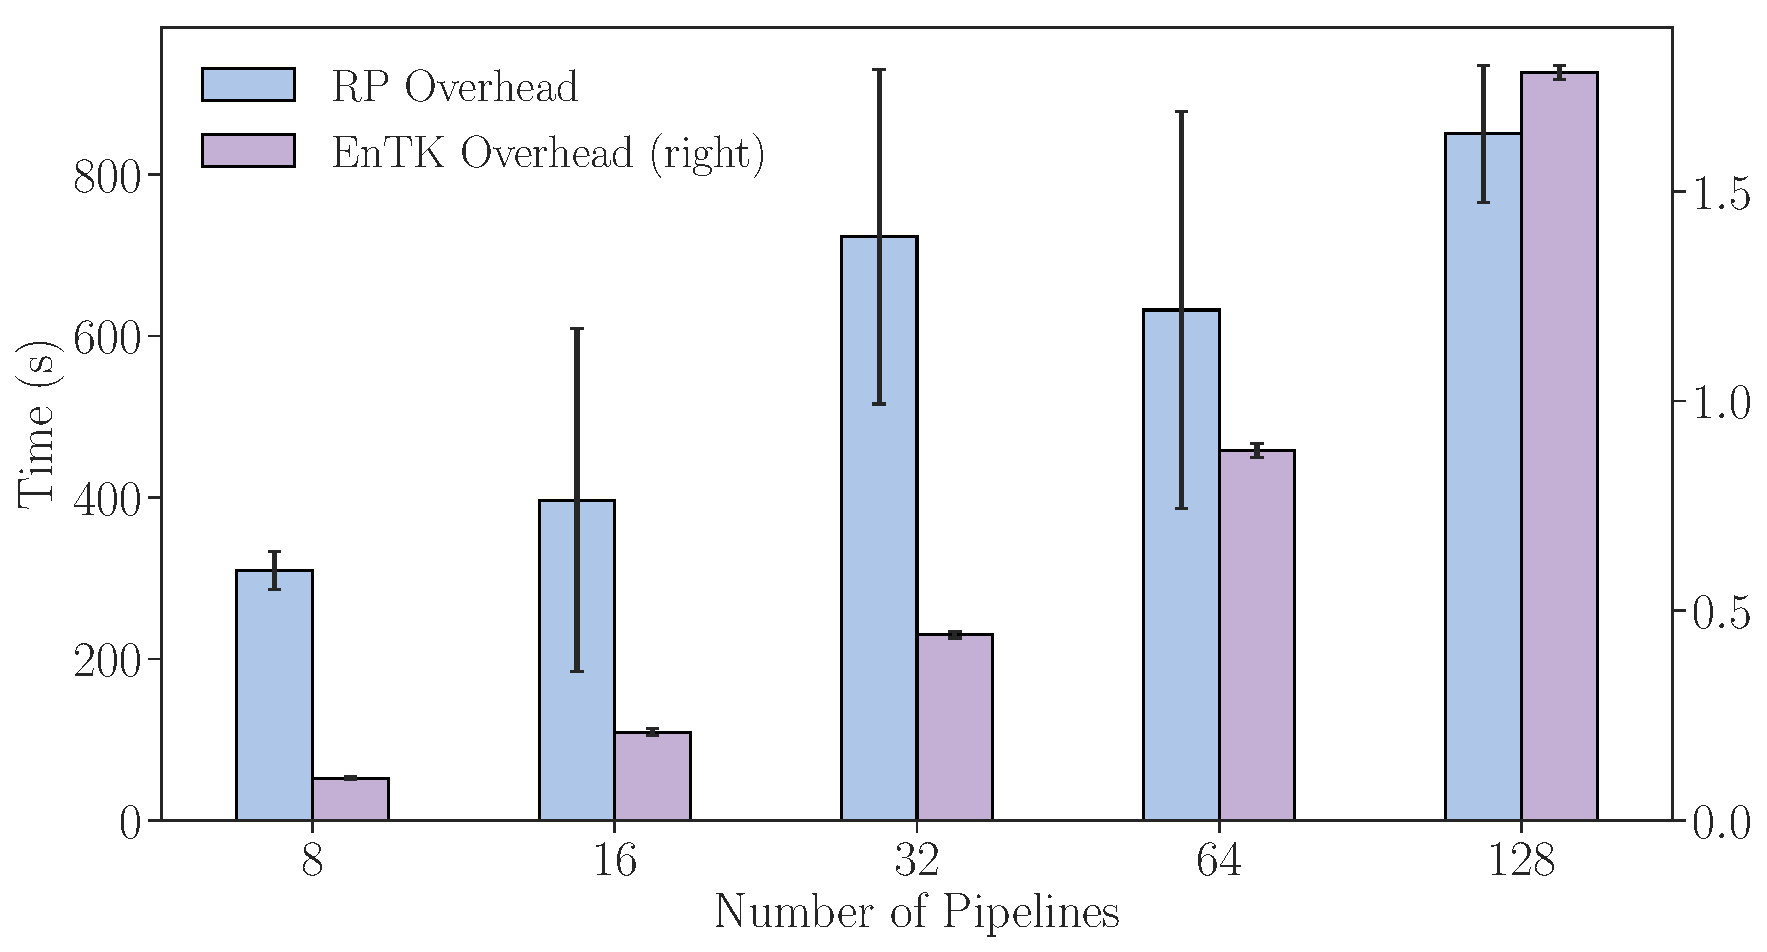
\includegraphics[width=\textwidth]{FIGURES/null_workload_overheads.pdf}
  \end{minipage}
  \begin{minipage}[b]{0.49\textwidth}
  \centering
  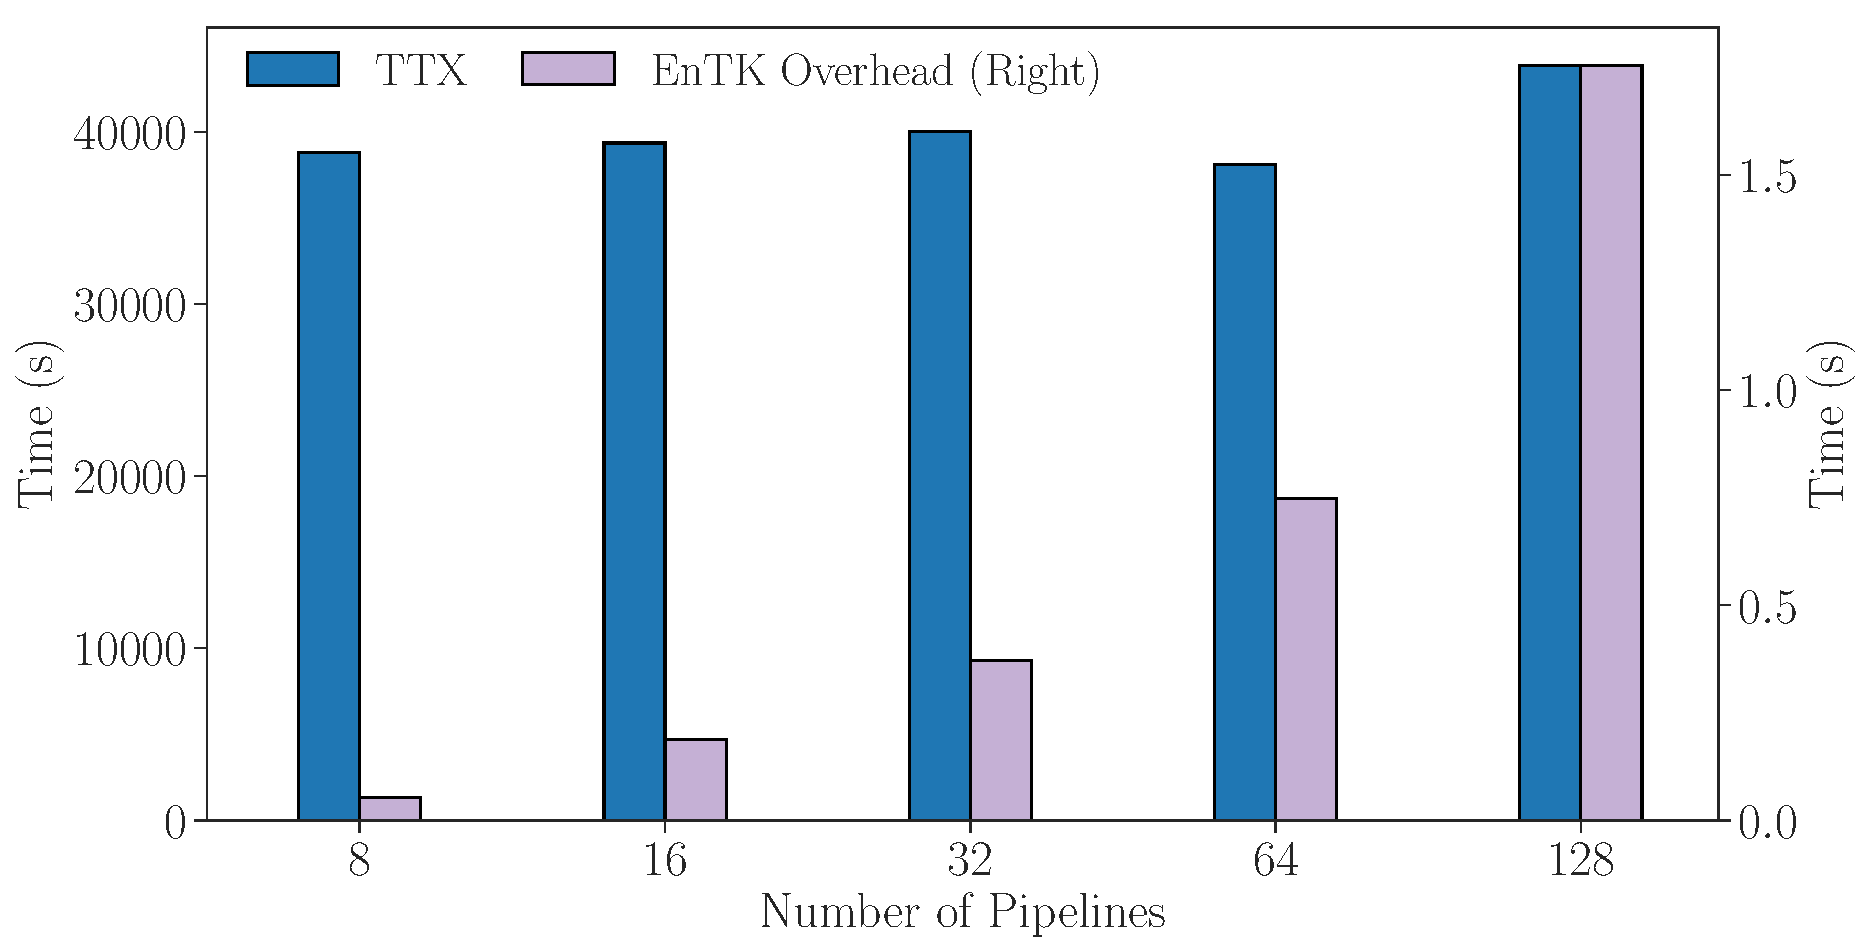
\includegraphics[width=\textwidth]{FIGURES/namd_workload_overheads.pdf}
  \end{minipage}
  \caption{\textbf{Top:} Weak scaling of HTBAC using null workload. We
          observe similar behavior at each configuration in the simulation
          execution time showing that the EnTK is invariant to the
          workload and a steady increase in the RP overhead due to the
          increase in the number of stages. \textbf{Bottom:} Weak scaling of
          HTBAC using use-case workload. We observe higher time-to-completions for each  than the null workload yet similar performance across pipelines indicating optimal weak scaling characterization.}\label{fig:htbac_perf}
\end{figure}


The fluctuation of the simulation execution times can be attributed to
run-time system fluctuations within the workload including stragglers at
higher pipeline and pipeline-to-pipeline fluctuations. In order to examine
the fluctuations within stages we corrolate the overhead for each pipeline at
the longest simulation duration in order to reconcile any fluctuations
induced by NAMD\@. We calculate time-to-execution (Tx) of the largest
pipeline size and compare the longest MD run within each pipeline. The NAMD
logs indicate a mean and variance as\ldots

% \begin{figure}[!htbp]
%   \centering
%   %\begin{minipage}[b]{0.6\textwidth}
%   \begin{minipage}[b]{0.55\textwidth}
%   \centering
%   %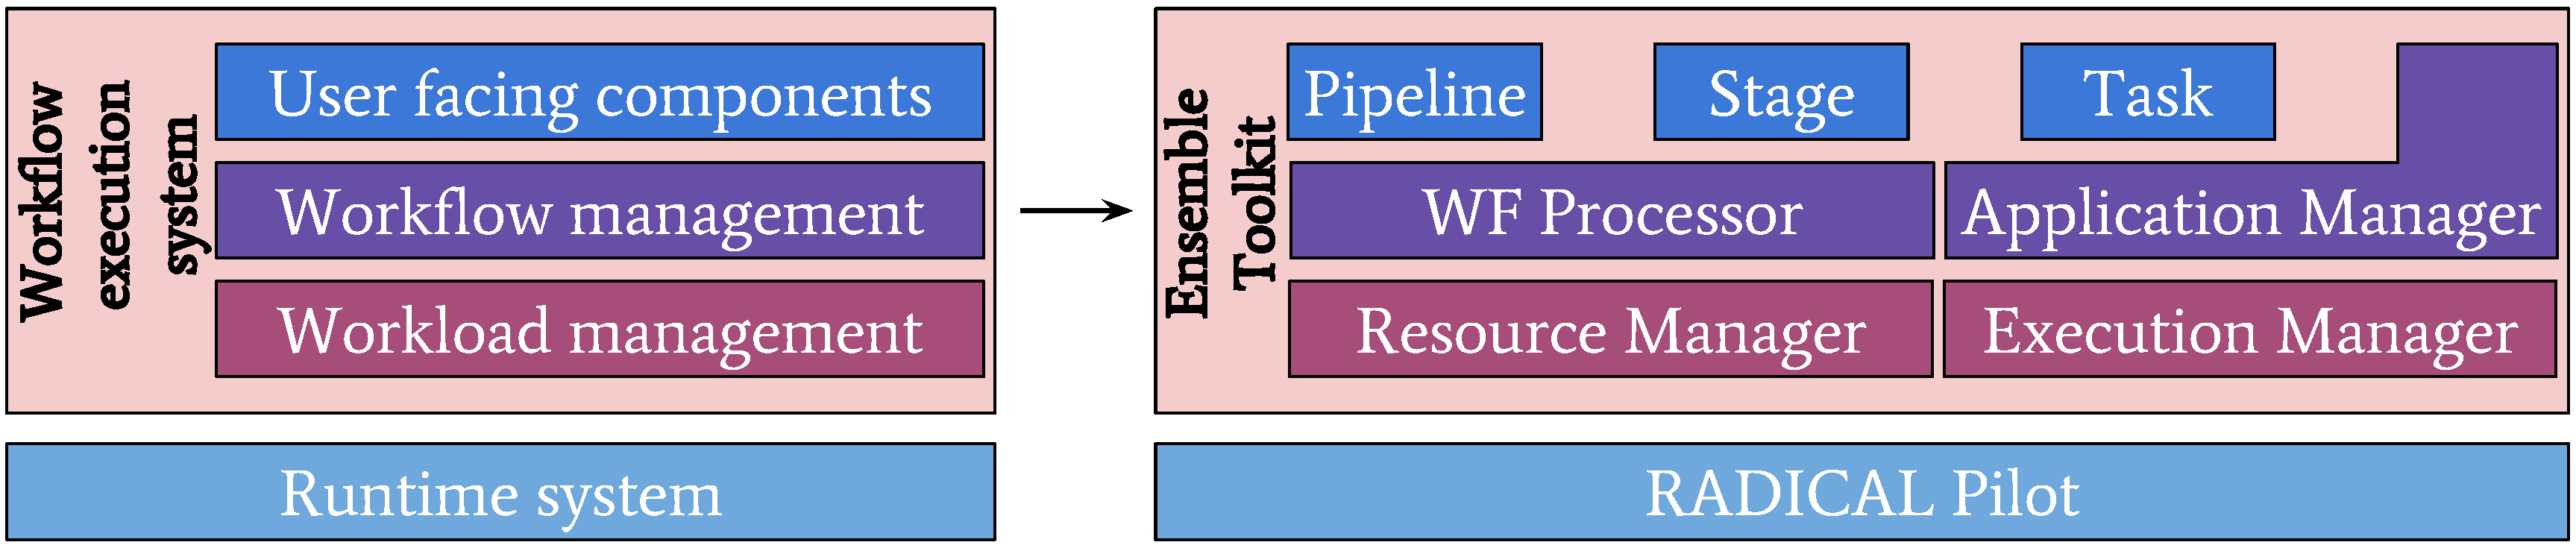
\includegraphics[width=\textwidth, height=35mm]{FIGURES/entk_overview.pdf}
% %  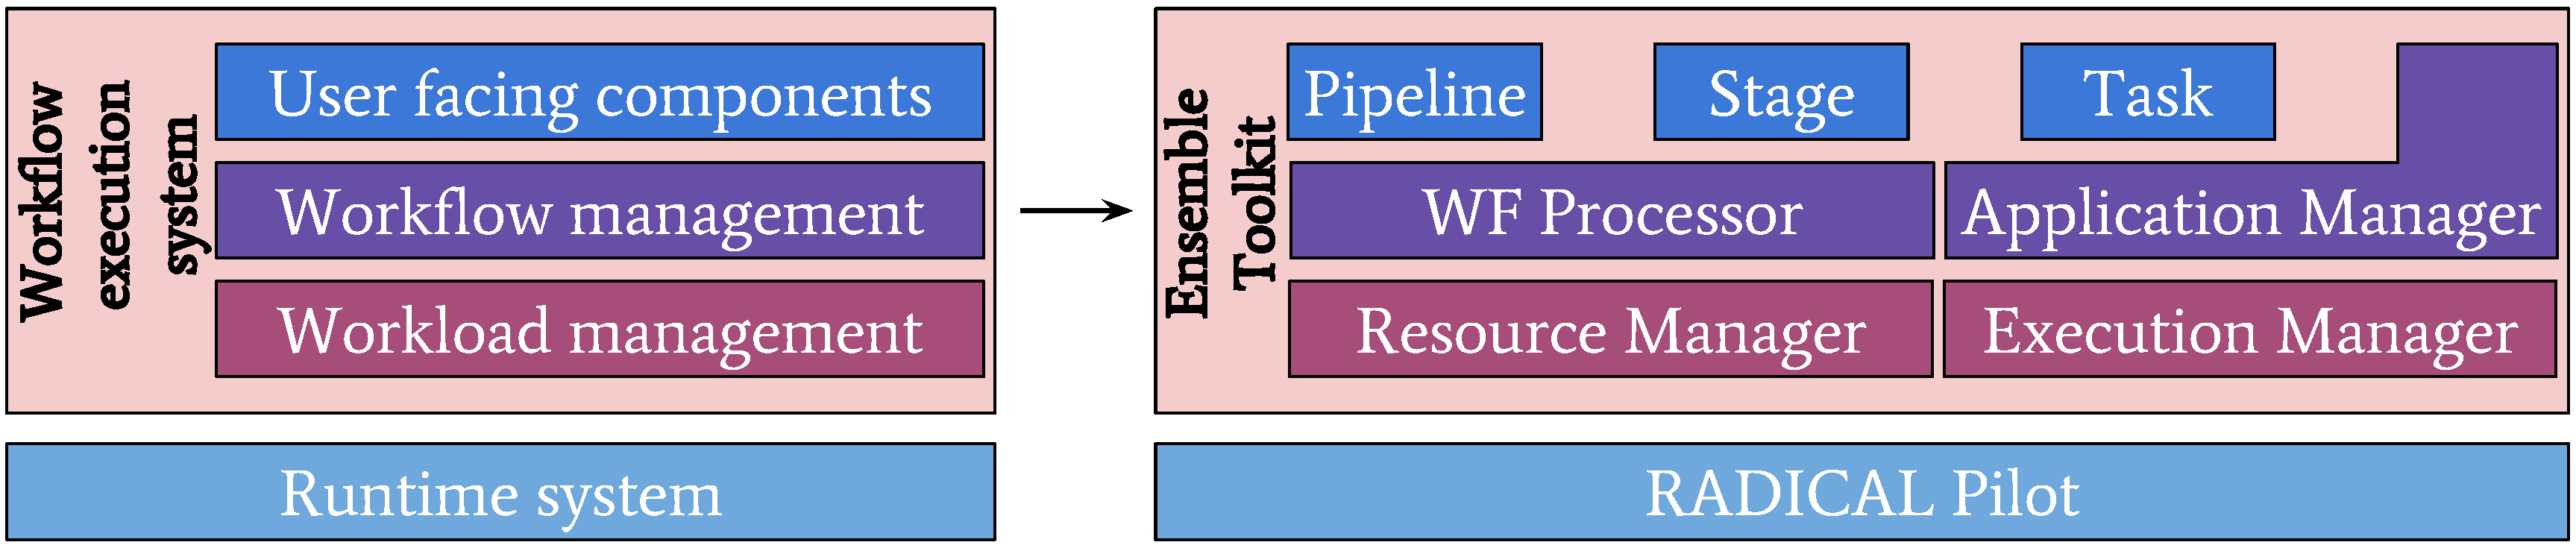
\includegraphics[width=\textwidth, height=40mm]{FIGURES/entk_overview.pdf}
%   \end{minipage}
%   %\begin{minipage}[b]{0.39\textwidth}
%   \begin{minipage}[b]{0.44\textwidth}
%   \centering
% %  \includegraphics[width=\textwidth, height=35mm]{FIGURES/md_general.pdf}
% %  \includegraphics[width=\textwidth, height=40mm]{FIGURES/md_general.pdf}
%   \end{minipage}
%   \caption{Overview of time-to-execution (Tx) of each pipeline at the
%            longest simulation duration as measured by NAMD log files,
%            showing how the distribution shows no abnormal fluctuations
%            across pipelines.}\label{fig:namd_logs}
% \end{figure}

\begin{figure}[!htbp]
  \begin{minipage}[b]{0.49\textwidth}
  \centering
  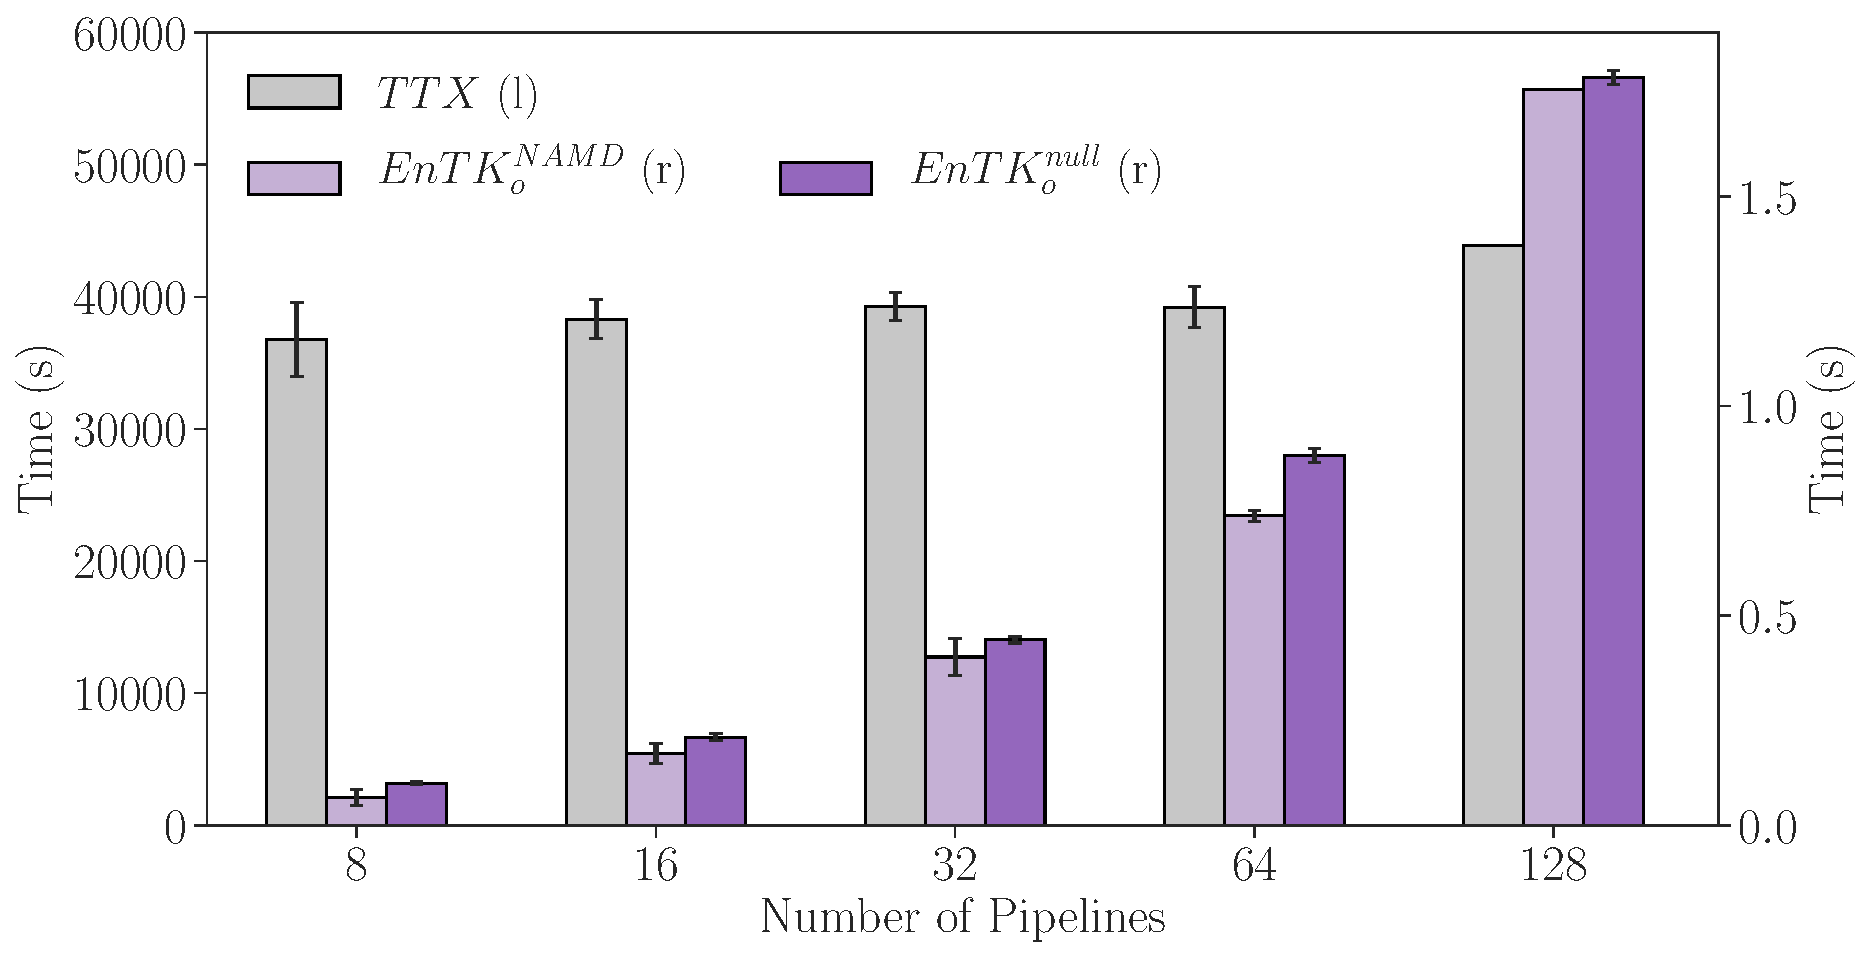
\includegraphics[width=\textwidth]{FIGURES/namd_null_workload_overheads.pdf}
  \end{minipage}
  \caption{EnTK overheads for null and NAMD workflows; no pilot overheads.}\label{fig:namd_logs}
\end{figure}


%NAMD logs - corrolate the overhead for each pipeline makes the system invariant to the worload. Remaining will be RP overhead. NAMD log files (utime) demonstrates time-to-execution (Tx) 

%Add in: what are the overheads, how is EnTK collecting overhead 




%eq0 : Minimize with decreasing restraints
%eq1 : NVT, 50K, with restraints
%eq2 : NPT, 300K, with decreasing restraints 
%sim1.conf: NPT, 300k, no constraints


%Need system verification of timestamps (errors) 




